\documentclass{standalone}
\usepackage{tikz}
\usepackage{pgfplots}
\usepgfplotslibrary{colormaps}
\pgfplotsset{colormap/copper2}

\begin{document}
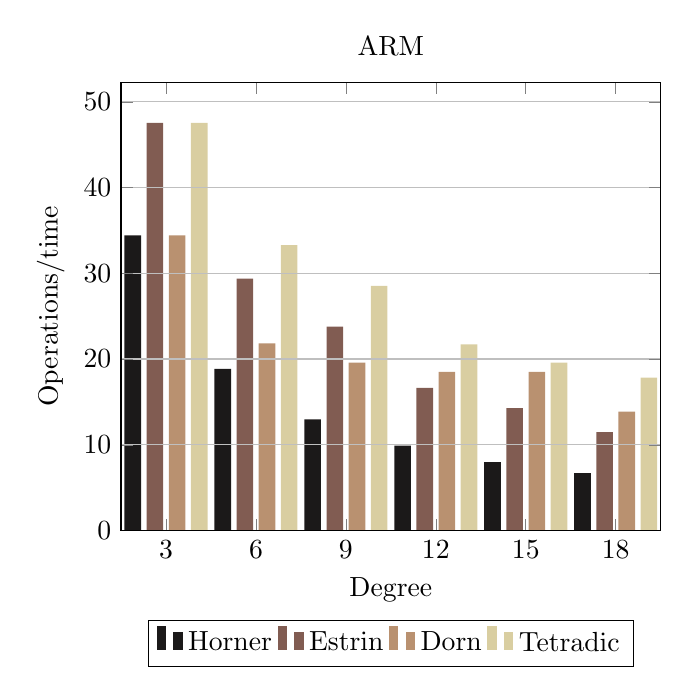
\begin{tikzpicture}

  \begin{axis}[
      ybar,
      axis on top,
      bar width=6pt,
      ymin=0,
      ymajorgrids,
      tick align=inside,
      xtick=data,
      symbolic x coords={3, 6, 9, 12, 15, 18},
      legend style={at={(0.5,-0.2)},anchor=north,legend columns=-1},
      title={ARM},
      xlabel={Degree},
      ylabel={Operations/time},
      colormap name=copper2
    ]
    % Horner
    \addplot [color of colormap={100},draw=none,fill=.] coordinates {
      (3, 34.43)
      (6, 18.85)
      (9, 12.97)
      (12, 9.89)
      (15, 7.99)
      (18, 6.7)
    };
    \addlegendentry{Horner};
    % Estrin
    \addplot [color of colormap={400},draw=none,fill=.] coordinates {
      (3, 47.54)
      (6, 29.37)
      (9, 23.78)
      (12, 16.65)
      (15, 14.27)
      (18, 11.48)
    };
    \addlegendentry{Estrin};
    % Dorn
    \addplot [color of colormap={600},draw=none,fill=.] coordinates {
      (3, 34.43)
      (6, 21.83)
      (9, 19.59)
      (12, 18.5)
      (15, 18.5)
      (18, 13.87)
    };
    \addlegendentry{Dorn};
    % Tetradic
    \addplot [color of colormap={800},draw=none,fill=.] coordinates {
      (3, 47.54)
      (6, 33.29)
      (9, 28.53)
      (12, 21.71)
      (15, 19.58)
      (18, 17.84)
    };
    \addlegendentry{Tetradic};
  \end{axis}

\end{tikzpicture}
\end{document}
